% Template from https://www.overleaf.com/latex/templates/international-university-hcmiu-vnu-pre-thesis-and-thesis-latex-template/hkwcgswxgfth

% Preamble
\documentclass[12pt, twoside]{report}

% Packages
\usepackage[utf8]{inputenc}
\usepackage{amsmath}
\usepackage{csquotes}
\usepackage{graphicx}
\usepackage[english]{babel}
\usepackage[a4paper, top=1in, bottom=0.8in, left=1in, right=1in]{geometry}
\usepackage{fancyhdr}
\usepackage[colorlinks=true,linkcolor=black]{hyperref}
\usepackage{comment}
\usepackage{float}
\usepackage{tikz}
\usepackage{tikz-qtree}
\usepackage{graphicx}
\usepackage{siunitx}

\usetikzlibrary{arrows,automata,positioning}

% Graphics path
\graphicspath{{images/}}

\begin{document}
	\pagenumbering{roman}

	% Title Page
	\begin{titlepage}

		\renewcommand{\thesection}{\arabic{section}}
		\newcommand{\HRule}{\rule{\linewidth}{0.2mm}}
		
		\center

		\textsc{\Large Ca' Foscari University of Venice }\\[1.0cm]
		\includegraphics[scale=0.85]{ unive-emblem.png }\\[1cm]
		\textsc{\Large Department of Environmental Sciences, Informatics and Statistics }\\[0.5cm]
		\textsc{\large MCS Computer Science and Information Technology CM-90 }\\[0.5cm]
		\textsc{\large [CM0481] Software Performance and Scalability }\\[0.5cm]
		
		\HRule \\[0.8cm]
		{ \Huge \bfseries IMDb: Performance and Scalability Analysis }\\[0.5cm]
		\HRule \\[0.8cm]
		
		\Large \emph{Authors:}\\
		Michele \textsc{Lotto} - {\normalsize 875922}\\
		Daniel Jader \textsc{Pellattiero} - {\normalsize 903837}\\[3.5cm]

		{\large Rev. 26/06/2024  }\\
		
		\vfill
		
	\end{titlepage}

	% Table of Contents, List of Figures, List of Tables
	\tableofcontents
	\listoftables
	\addcontentsline{toc}{chapter}{List of Tables}
	\listoffigures
	\addcontentsline{toc}{chapter}{List of Figures}

	% Abstract
	\chapter*{Abstract}
	\addcontentsline{toc}{chapter}{Abstract}
	This report presents a comprehensive account of the implementation and performance testing process conducted on a web application that emulates the IMDb website\footnote[1]{https://www.imdb.com/}.

The report begins with an overview of the system implementation, in which the technologies utilised are outlined. Subsequently, a theoretical analysis of the queueing system network is presented, in which the implemented system is characterised.
The load test conducted on the system will be subjected to a thorough examination, including an analysis of its theoretical and empirical findings.

In conclusion, a potential architectural solution is evaluated for its potential to enhance the scalability of the tested system.

It should be noted that the implementation of the system, along with all automated programs and scripts referenced in this report, is fully documented and accessible on the GitHub repository\footnote[2]{https://github.com/danieljaderpellattiero/unive-imdb}.


	% Body of the paper
	\chapter{System implementation}
	\pagenumbering{arabic}
	\setcounter{page}{1}
	% Chapter introduction

The project entails the development of a three-tiered web application, comprising a database, a RESTful API and a website.
The following sections will present an analysis of each of these components, with a focus on the technologies and design choices implemented.

\section{Database -- MongoDB}

MongoDB is a popular NoSQL document-oriented database that is designed to store and manage large volumes of structured and unstructured data.

The database was selected as the optimal choice for managing the IMDb Non-Commercial Datasets\footnote[1]{https://developer.imdb.com/non-commercial-datasets/} due to its adoption of a schemaless data modelling, which enables the management of any non-normalised records or fields within the data.
Furthermore, the usage of JSON format for storing the records allows for enhanced efficiency in interactions with the backend.

\subsection{Data analysis}

Each dataset, comprising a UTF-8-encoded tab-separated values (TSV) file, was subjected to analysis using the Python \verb|Pandas| library.
The primary steps of the data analysis process were as follows:

\begin{enumerate}
	\item The replacement of missing values (denoted by  \verb|`\N'|) with default values of a type consistent with the column domain to which they belong.
	\item The removal of records that lack some data fields.
	\item The normalisation of fields containing arrays of elements.
	\item The potential replacement of table indexes.
\end{enumerate}

Further modifications were implemented to the tables, however, as these affect the database schema, they will be addressed subsequently.

Once the preliminary phase of preparing the datasets was complete, it was decided that the files should be exported in the JSON format, allowing them to be imported into the database.
Additionally, the files were exported also in the Parquet format, enabling them to be uploaded to the GitHub repository via the GitHub Large File Storage (LFS) facility\footnote[2]{https://git-lfs.com/}. 

\subsection{Collections' schema}

MongoDB represents objects using BSON (Binary JSON) types, which are binary-encoded serialisations of documents that adhere to the JSON format.
As each table in MongoDB is translated into the concept of a document collection, the diagrams of the respective collections imported from the datasets obtained post data analysis are presented below.
Furthermore, supplementary notes on the refactoring of the tables are provided.

\begin{table}[H]
	\caption{`\textit{title.basics}' collection schema}
\begin{center}
	%\def\arraystretch{1.4}
	\begin{tabular}{ cccc }
		%\multicolumn{5}{c}{} \\
		\hline
		Field & BSON type & Index & Index type \\
		\hline
		\_id & String & yes & unique, ascending \\
		titleType & String & no & - \\
		name & String & no & - \\
		nameEng & String & no & - \\
		isAdult & Boolean & no & - \\
		genres & Array[String] & no & - \\
		startYear & 32-bit integer & no & - \\
		endYear & 32-bit integer & no & - \\
		runtime & 32-bit integer & no & - \\
		rating & Double & no & - \\
		votes & 32-bit integer & no & - \\
		\hline
	\end{tabular}
\end{center}
\end{table}  

\textit{N.d.R.}: A collection was created ad hoc for records with the field \textit{`titleType'} equal to \textit{`tvEpisode'}.

\begin{table}[H]
	\caption{`\textit{title.akas}' collection schema}
\begin{center}
	%\def\arraystretch{1.4}
	\begin{tabular}{ cccc }
		%\multicolumn{5}{c}{} \\
		\hline
		Field & BSON type & Index & Index type \\
		\hline
		\_id & ObjectId & yes & unique, ascending \\
		titleId & String & no & - \\
		ordering & 32-bit integer & no & - \\
		region & String & no & - \\
		name & String & no & - \\
		nameLower & String & yes & ascending \\
		\hline
	\end{tabular}
\end{center}
\end{table}

\textit{N.d.R.}: \textit{`language'}, \textit{`types'}, \textit{`attributes'}, \textit{`isOriginalTitle'} fields dropped.

\begin{table}[H]
	\caption{`\textit{title.crew}' collection schema}
\begin{center}
	%\def\arraystretch{1.4}
	\begin{tabular}{ cccc }
		%\multicolumn{5}{c}{} \\
		\hline
		Field & BSON type & Index & Index type \\
		\hline
		\_id & String & yes & unique, ascending \\
		writers & Array[String] & no & - \\
		directors & Array[String] & no & - \\
		\hline
	\end{tabular}
\end{center}
\end{table}

\begin{table}[H]
	\caption{`\textit{title.episodes}' collection schema}
\begin{center}
	%\def\arraystretch{1.4}
	\begin{tabular}{ cccc }
		%\multicolumn{5}{c}{} \\
		\hline
		Field & BSON type & Index & Index type \\
		\hline
		\_id & String & yes & unique, ascending \\
		titleId & String & yes & ascending \\
		name & String & no & - \\
		nameEng & String & no & - \\
		season & 32-bit integer & no & - \\
		episode & 32-bit integer & no & - \\
		isAdult & Boolean & no & - \\
		genres & Array[String] & no & - \\
		startYear & 32-bit integer & no & - \\
		endYear & 32-bit integer & no & - \\
		runtime & 32-bit integer & no & - \\
		rating & Double & no & - \\
		votes & 32-bit integer & no & - \\
		\hline
	\end{tabular}
\end{center}
\end{table}

\begin{table}[H]
	\caption{`\textit{name.basics}' collection schema}
	\begin{center}
		%\def\arraystretch{1.4}
		\begin{tabular}{ cccc }
			%\multicolumn{5}{c}{} \\
			\hline
			Field & BSON type & Index & Index type \\
			\hline
			\_id & String & yes & unique, ascending \\
			fullName & String & no & - \\
			birth & 32-bit integer & no & - \\
			death & 32-bit integer & no & - \\
			professions & Array[String] & no & - \\
			\hline
		\end{tabular}
	\end{center}
\end{table}

\textit{N.d.R.}: \textit{`knownForTitles'} field dropped.

\begin{table}[H]
	\caption{`\textit{title.principals}' collection schema}
\begin{center}
	%\def\arraystretch{1.4}
	\begin{tabular}{ cccc }
		%\multicolumn{5}{c}{} \\
		\hline
		Field & BSON type & Index & Index type \\
		\hline
		\_id & ObjectId & yes & unique, ascending \\
		titleId & String & yes & ascending \\
		ordering & 32-bit integer & no & - \\
		personId & String & no & - \\
		job & String & no & - \\
		characters & Array[String] & no & - \\
		\hline
	\end{tabular}
\end{center}
\end{table}

\textit{N.d.R.}: \textit{`category'} field used to fill empty \textit{`job'} fields; then dropped.

\subsection{Schema indexes and bulk data insert}

As can be seen from the tables above, in addition to the standard unique indexes, it was decided to add additional ones to optimise the queries requested by the backend.
Given the significant use of wildcard searches based on regular prefix expressions, it was decided to implement ascending indexes on several \textit{`String'} type fields to drastically reduce search times without having to resort to a text index, which would take up much more space due to the tokenisation and stemming of the fields.

In order to perform a bulk insert of the approximately 42.5 million records contained in $\sim1.6$ GB of JSON files, it was decided to write a script in Python that would take advantage of a multithreaded execution of the \verb|mongoimport| command-line tool provided by MongoDB.
The overall script is responsible for generating the database's collections, populating them and finally creating indexes.

\subsection{Technical details}

The database was configured as a locally managed instance of MongoDB, thus avoiding the utilisation of the cloud version of the service (Atlas).
The service's local deployment facilitated the monitoring and control of its resources, as well as the measurement of its performance.
These factors collectively contributed to the generation of more reliable results during the load tests that were conducted.

Technical insights into the environment are presented below.

\begin{itemize}
	\item MongoDB 7.0.11 (Community Server service)
	\item MongoDB Compass 1.43.3 (database UI)
	\item MongoDB Shell 2.2.9 (database CLI)
\end{itemize}

\section{RESTful API -- Express}

The web application's backend was developed using the Express framework, a Node.js web application framework that was identified as the most widely utilised in the ``State of JavaScript 2023'' survey\footnote[3]{https://2023.stateofjs.com/en-US/other-tools/\#backend\_frameworks}.

A variety of endpoints were incorporated into the API, enabling a constrained yet still functional utilisation of the web interface.
The user-accessible API calls are enumerated below, along with a concise description of each.

\begin{enumerate}
	\item \verb|localhost:3000/search/preview/:title| -- Returns the top 4 most voted titles that match the search query prefix.
	\item \verb|localhost:3000/search/:title| -- Returns the most voted titles that match the search query prefix; the results are paginated in groups of 8.
	\item \verb|localhost:3000/search/episodes/:title| -- Returns the episodes of a specific title that matches the \textit{`titleId'} parameter.
	\item \verb|localhost:3000/title/:id| -- Returns the details of a specific title that matches the \textit{`\_id'} parameter.
	\item \verb|localhost:3000/episode/:id| -- Returns the details of a specific episode that matches the \textit{`\_id'} parameter.
\end{enumerate}

The official MongoDB driver for Node.js (Typescript) \verb|mongodb@6.8| is responsible for handling queries from the backend to the database.
We deliberately decided not to utilise any form of Object-Relational/Document Mapping (e.g. \verb|Mongoose| or \verb|Prisma|) due to the suitability of the JSON record format to the application domain model and potential performance overheads.

Aggregation pipelines are used to facilitate the execution of queries to the database.
These pipelines allow the definition of queries through the use of a sequential list of stages, thereby simplifying the grouping and sorting of data and providing control over the execution times of the individual stages within the pipeline.

\section{Website -- Vue and Tailwind CSS}

The web interface of the system was realised using Vue.js ``The Progressive JavaScript Framework'', a well-known framework used for building SPAs (Single Page Applications) renowned for its component-based architecture and reactive data binding system.
The aesthetic component was addressed through the utilisation of Tailwind CSS, a utility-first CSS framework that can be suitably integrated with Vue.
A bundle of the website, optimised for deployment on a static hosting service, was created at the end of the development process using Vite\footnote[4]{A modern front-end build tool that facilitates optimised production builds through the utilization of ES hot module replacement (HMR).}.
This design choice ensures that the frontend is efficiently packaged into static files, which can be served directly to users without requiring server-side processing.
Consequently, during load testing with JMeter, the focus has been exclusively on the backend API endpoints, as the frontend's static nature does not impose additional load on the server.

Thumbnails of the web interface are available on GitHub\footnote[5]{https://github.com/danieljaderpellattiero/unive-imdb/tree/frontend/thumbnails}.


	\chapter{Test case identification}
	\section{High-level design}

This brief chapter aims to present the test case designed to perform the load test of the system.
In order to illustrate the user behaviour modelled by the test, we define a trivial finite-state automata with reference to the endpoints implemented in the RESTful API.

It should be noted that, although this aspect will be discussed in greater detail in the following chapters, the two endpoints that will be used in the load test result in two different classes of jobs, which must consequently be analysed individually.

\begin{center}
	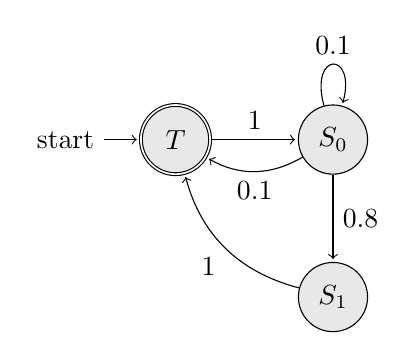
\begin{tikzpicture}[shorten >=1pt,node distance=2cm,on grid,auto]
		\tikzstyle{every state}=[fill={rgb:black,1;white,10}]
		\node[state, initial, accepting] (0) {$T$};
		\node[state] (1) [right of = 0] {$S_0$};
		\node[state] (2) [below of = 1] {$S_1$};
		\path[->]
		(0) edge node {1} (1)
		(1) edge [loop above] node {0.1} (1)
		(1) edge [bend left] node {0.1} (0)
		(1) edge node {0.8} (2)
		(2) edge [bend left] node {1} (0);
		;
	\end{tikzpicture}
\end{center}

The above automata has to be interpreted in the following manner:

\begin{itemize}
	\item The user initiates a title search by name match, regardless of the customer language locale. (\verb|/search/:title| -- node $S_{0}$)
	\begin{itemize}
		\item In $80\%$ of cases, the search continues with a precise request for the title information. (\verb|/title/:id| \textit{or} \verb|/episode/:id| -- node $S_{1}$)
		\item In $20\%$ of cases, either the user terminates the search process pre-emptively, without finding the title, thus entering a thinking state (node $T$) or it continues the search by hitting the same endpoint though the use of pagination. (\verb|/search/:title?page=n| -- node $S_{0}$)
	\end{itemize}
	\item Upon receipt of the searched title information, the user is satisfied and returns to the thinking state before repeating a new search.
\end{itemize}

\clearpage

\section{Computational settings}

The following table provides an overview of the hardware specifications of the computers utilised in the load test.

\begin{table}[H]
	\caption{Hardware specifications}
\begin{center}
	%\def\arraystretch{1.4}
	\begin{tabular}{ ccccc }
		%\multicolumn{5}{c}{} \\
		\hline
		Machine type & Role & O.S. & CPU & RAM \\
		\hline
		Desktop & Benchmark executor & Ubuntu 22.04 & Intel i5-13600K (20) & 64 GB \\
		Laptop & System under test & Ubuntu 22.04 & Intel i5-8265U (8) & 8 GB \\
		\hline
	\end{tabular}
\end{center}
\end{table}


	\chapter{Queueing network model}
	\section{Introduction}

This chapter presents a comprehensive theoretical analysis of the implemented model.
The following illustration depicts the system components involved in the load test in the context of queuing theory. 

For the purposes of this illustration, let Q\textsubscript{T} represent the thinking station, Q\textsubscript{B} represent the backend, and Q\textsubscript{D} represent the database.

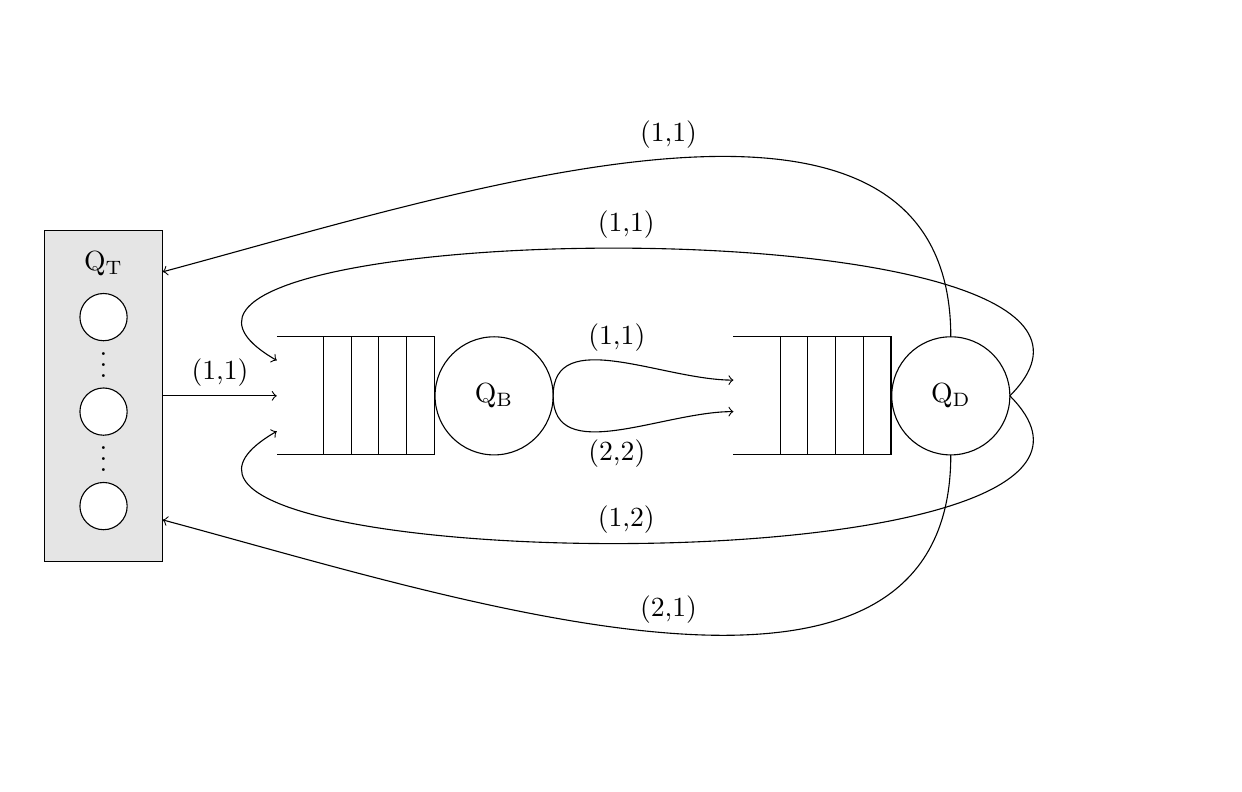
\begin{tikzpicture}
	\tikzstyle{thinking_station} = [rectangle, draw, minimum height=4.2cm, minimum width=1.5cm, fill=gray!20, align=left]
	\tikzstyle{circle_node} = [circle, draw, fill=white, minimum size=6mm, inner sep=0pt]
	\tikzstyle{queue} = [circle, draw, minimum size=1cm, text centered, inner sep=0pt]

	% Thinking station
	\node (QT) [thinking_station] at (0,0) {};
	\node at (0,1.68) {Q\textsubscript{T}};
	% Users belonging to the closed loop
	\node[circle_node] at (0, 1) {};
	\node at (0, 0.5) {$\vdots$};
	\node[circle_node] at (0, -0.2) {};
	\node at (0, -0.7) {$\vdots$};
	\node[circle_node] at (0, -1.4) {};

	% Backend station
	% Queue
	\draw (2.2,0.75) -- ++(2cm,0) -- ++(0,-1.5cm) -- ++(-2cm,0);
	\foreach \i in {1,...,4}
	\draw (4.2cm-\i*10pt,0.75) -- +(0,-1.5cm);
	% Service room
	\draw (4.96,-0.00cm) circle [radius=0.75cm];
	% Label service time
	\node at (4.96,-0.00cm) {Q\textsubscript{B}};

	% Database station
	% Queue
	\draw (8.0,0.75) -- ++(2cm,0) -- ++(0,-1.5cm) -- ++(-2cm,0);
	\foreach \i in {1,...,4}
	\draw (10cm-\i*10pt,0.75) -- +(0,-1.5cm);
	% Service room
	\draw (10.760,-0.00cm) circle [radius=0.75cm];
	% Label service time
	\node at (10.760,-0.00cm) {Q\textsubscript{D}};

	\draw[->]	(QT) to[out=0,in=180] node[above]	{(1,1)} (2.2,0);
	\draw[->]	(5.71,0) to[out=90,in=180] node[above]	{(1,1)} (8.0,0.20);
	\draw[->]	(5.71,0) to[out=-90,in=180] node[below]	{(2,2)} (8.0,-0.20);
	\draw[->]	(11.51,0) to[out=45,in=150] node[above]	{(1,1)} (2.2,0.45);
	\draw[->]	(11.51,0) to[out=-45,in=-150] node[above]	{(1,2)} (2.2,-0.45);
	\draw[->]	(10.760,-0.75) to[out=-90,in=-15] node[above]	{(2,1)} (0.75,-1.575);
	\draw[->]	(10.760,0.75) to[out=90,in=15] node[above]	{(1,1)} (0.75,1.575);
\end{tikzpicture}

It is possible to derive several characteristics of the system under consideration from the illustration above.

The system is characterised by a closed and interactive nature, free of stability conditions, and a constant number of users that dictate the nature of the workload.
A further aspect that emerges relates to the multiclass nature of the jobs within the system, as indicated by the labels placed at the station entry and exit arcs.

Subsequently, an in-depth examination will be conducted on the distinct service time/demand and probabilistic routing for the two classes of jobs.

In conclusion, the network under analysis can be classified as a BCMP, exhibiting a closed topology and utilising ``Processor Sharing'' (PS) as its scheduling discipline.

Prior to examining the nature of the queues that characterise our network and their associated scheduling disciplines, we proceed with the formalisation and resolution of the network's traffic equations.
These equations will then be essential in producing the theoretical analysis of the system.

\section{Traffic equations}

The system's traffic equations are presented below.

\[
	\begin{array}{c}
	\begin{bmatrix}
	p_{T1B1} \\
	p_{B1D1} \\
	p_{B2D2} \\
	p_{D1B1} \\
	p_{D1B2} \\
	p_{D1T1} \\
	p_{D2T1}
	\end{bmatrix}
	=
	\begin{pmatrix}
	1.0 \\
	1.0 \\
	1.0 \\
	0.1 \\
	0.8 \\
	0.1 \\
	1.0
	\end{pmatrix}
	\end{array}
	\quad : \quad
	\begin{cases}
	\begin{aligned}
	e_{B1} &= e_{T1} + (p_{D1B1} \times e_{D1}) \\
	e_{B2} &= p_{D1B2} \times e_{D1} \\
	e_{D1} &= e_{B1} \\
	e_{D2} &= e_{B2} \\
	e_{T1} &= e_{D2} + (p_{D1T1} \times e_{D1}) \\
	\end{aligned}
	\end{cases}
	\Rightarrow
	\begin{cases}
	\begin{aligned}
	% Insert your new system here, for example:
	e_{B1} &= \num[round-mode=places, round-precision=4]{1.11111111111111} \times e_{T1}  \\
	e_{B2} &= \num[round-mode=places, round-precision=4]{0.888888888888889} \times e_{T1}  \\
	e_{D1} &= \num[round-mode=places, round-precision=4]{1.11111111111111} \times e_{T1}  \\
	e_{D2} &= \num[round-mode=places, round-precision=4]{0.888888888888889} \times e_{T1}  \\
	\end{aligned}
	\end{cases}
\]

The system of equations above demonstrates that our routing is irreducible, which implies that any queue can be accessed from any other queue within the network.
From an analytical standpoint, our system is under-determined, indicating the existence of an infinite number of solutions. The non-trivial solutions can be derived from the non-zero multiplicative coefficients.

Moreover, it is essential to highlight that within this context, where the system under consideration is an interactive queueing network, it is imperative to impose an additional constraint on the previous system, specifically $e_{T1}=1$, given that this is the thinking station Q\textsubscript{T}.

\section{Queueing network components}

This section will provide a brief overview of the components of our network, with reference to Kendall's notation.

\subsection{Thinking station}

The thinking station can be represented by a queuing system described with the \newline ``G/D/$\infty$/IS'' notation.
The distribution of inter-arrival times for jobs at the thinking station is unknown, but the distribution of service times is known, as the jobs within it remain in service (\textit{thinking state}) for a fixed constant time, known as thinking time.
By definition, the thinking station is equipped with an infinite number of servers, indeed an undefined number of jobs can access it.
Consequently, the service discipline of this system is of the ``Delay center'' or ``Infinite Servers'' type, as all the jobs remain in an idle state in parallel.

\subsection{Backend station}

With regard to the JavaScript runtime environment Node.js, despite its reputation as a ``purely single-threaded'' execution environment due to its Event Loop, it is in fact capable of offloading I/O blocking operations to separate threads or the operating system, thus allowing the main thread to continue processing other tasks.
The library that permits the dispatching of blocking operations to a thread pool is called \verb|libuv| and it belongs to the Chrome V8 Engine.
Furthermore, Node.js has also implemented the \verb|worker_threads| module, which allows for further enhancements of performance by the utilisation of multi-core processors for CPU-bound operations.

In light of the aforementioned considerations, it can be concluded that the RESTful API functions as a ``G/G/1/PS'' queueing system.
This is due to the fact that no manual instantiation of multiple worker threads was performed for the API, and thus a unique main thread is responsible for handling all incoming requests through a ``Processor Sharing'' scheduling discipline.

\subsection{Database station}

With regard to MongoDB, an examination of the ``Production Notes'' section reveals that its WiredTiger storage engine is inherently multithreaded.
In particular, the total number of active threads (i.e. concurrent operations) relative to the number of available CPUs can impact performance as follows:

\begin{itemize}
	\item The throughput increases in direct proportion to the number of concurrent active operations, up to the overall number of CPUs.
	\item The throughput decreases as the number of concurrent active operations exceeds the number of CPUs by a certain threshold amount.
\end{itemize}

The optimal number of concurrent active operations for a given application can be determined through the measurement of throughput.

In order to ascertain the exactness of the information provided in the documentation, an empirical test was conducted to monitor the thread pool instantiated by the MongoDB service in both idle and stressed states.

The results obtained from the Linux command-line utility \verb|htop| are presented below.

\begin{figure}[h]
    \centering
    \includegraphics[width=\linewidth]{003/mongo-idle.png}
    \caption{MongoDB thread pool in idle state}
\end{figure}

\begin{figure}[h]
	\centering
	\includegraphics[width=\linewidth]{003/mongo-stress.png}
	\caption{MongoDB thread pool under load conditions}
\end{figure}	

In conclusion, the database can be identified as a ``G/G/\#C/PS'' queueing system, where ``\#C'' represents the number of cores.
The inter-arrival times and service times are both unknown, however it can be stated that the database leverages all CPU cores with a ``Processor Sharing'' service discipline.


	\begin{comment}
	Capitolo 4: Queueing network theoretical analysis
		- Service times measurements.
		- Bottleneck identification.
		- Mean Value Analysis.
			- Throughput over # users. (+ graphic)
			- Response time over # users. (+ graphic)
		- Asymptitic bounds and optimal number of users.
			- Bounds calculation.
			- Throughput over # users with bounds. (+ graphic)
			- Response time over # users with bounds. (+ graphic)
			- Optimal number of users.
	Capitolo 5: Experimental network analysis
		- Illustrazione load test JMeter.
		- Spiegazione configurazione del load test.
		- Grafici throughput e response time arricchiti.
	Capitolo 6: Results comparison
		- Confronto analisi teorica e sperimentale.
	Capitolo 7: Conclusioni
		- Proposta di architettura scalabile.
			- MongoDB caching.
			- MongoDB Sharding e replica.
			- Analisi prestazioni sistema proposto con MVA.
	\end{comment}

\end{document}
